\documentclass[../summary.tex]{subfiles}

\begin{document}
	
	\section{Buildings}
	
	\subsection{Study guide}
	
	Module 8 on Buildings sketches basic insights into the environmental impact of buildings and their role in a transition towards a more sustainable society. 
	
	\begin{itemize}
		\item You should clearly understand the concepts discussed in the module, be able to recognize examples, and be able to read the diagrams.
		\item Important concepts: role of buildings in reducing the environmental impact, existing policy on energy performance of buildings, life cycle of a building, life cycle assessment, operational and embodied carbon, carbon footprint and ecological footprint, life cycle financial impact of buildings, possible solutions for building renovation, possible solutions to reduce the environmental impact of buildings, urbanization and urban heat island.
		\item It is not necessary to memorize the numerical values shown in the diagrams, but it is necessary to understand the meaning of the diagrams.
	\end{itemize}
	
	\subsection{Environmental impact of construction}
	\subsubsection{Context}
	
	\textbf{The building sector is responsible for 40\% of the energy use and 36\% of greenhouse gas emissions. The building sector hence plays an important role in climate change}. Besides the global impact of these greenhouse gas emissions, these cause local effects as well. In cities, temperatures are rising and are typically higher than in suburban areas. This is called the \textbf{heat-island effect} and is caused by higher absorption of solar radiation by buildings and infrastructure. To date 55\% of the global population lives in cities and it is expected that this will increase to about 70\% by 2050, this is called \textbf{urbanization}.
	\\\\	
	To reduce the \textbf{impact of buildings on climate change}, important steps have been taken. In 2010, the \textbf{European Commission introduced a directive on the energy performance of buildings} that requires that all \textbf{new buildings have to be nearly-zero energy}. This resulted in a transition of buildings, where the buildings today are well insulated, air-tight, ventilated and are foreseen of at least a share of renewable energy to fulfil the nearly-zero-energy requirements. 
	
	\subsubsection{Main challenges}
	
	To reduce this environmental impact, we are facing \textbf{various challenges}. A first important challenge is \textbf{reducing the energy use of existing buildings}. These buildings are not well insulated and require an in-depth renovation. To reach the European climate goals, the renovations should be \textbf{deep energetic renovations}. This means that replacing windows or adding roof insulation is insufficient. By re-using the demolished parts of the buildings, we can reduce the need for virgin resources. \textbf{Buildings should hence be seen as material banks}, enabling urban mining.
	\\\\
	A second challenge relates to the need to \textbf{reduce embodied impacts}. These are \textbf{the greenhouse gas emissions due to the production, transport and end-of-life treatment of materials}. So far, the main efforts to reduce the climate change impact of buildings focused on reducing the operational energy use of buildings. To further reduce the carbon footprint of buildings, it is hence \textbf{important to not solely focus on the operational phase} (blue blocks on figure \ref{fig:8-embodied-operational-trends}), \textbf{but also take into account the embodied impact} (red blocks on figure \ref{fig:8-embodied-operational-trends}). \\
	If not, this could lead to a burden shifting from the operational to embodied carbon, potentially resulting in higher life cycle emissions. For newly built nearly-zero energy buildings, the \textbf{embodied emissions have become evenly important as the operational emissions}. This is visualized by the dashed line on figure \ref{fig:8-embodied-operational-trends}. The majority of the embodied emissions occur at the moment of renovation or construction, these are called \textbf{‘up-front’ emissions}. Reducing the upfront emissions is more urgent.
	
	\begin{figure}[H]
		\centering
		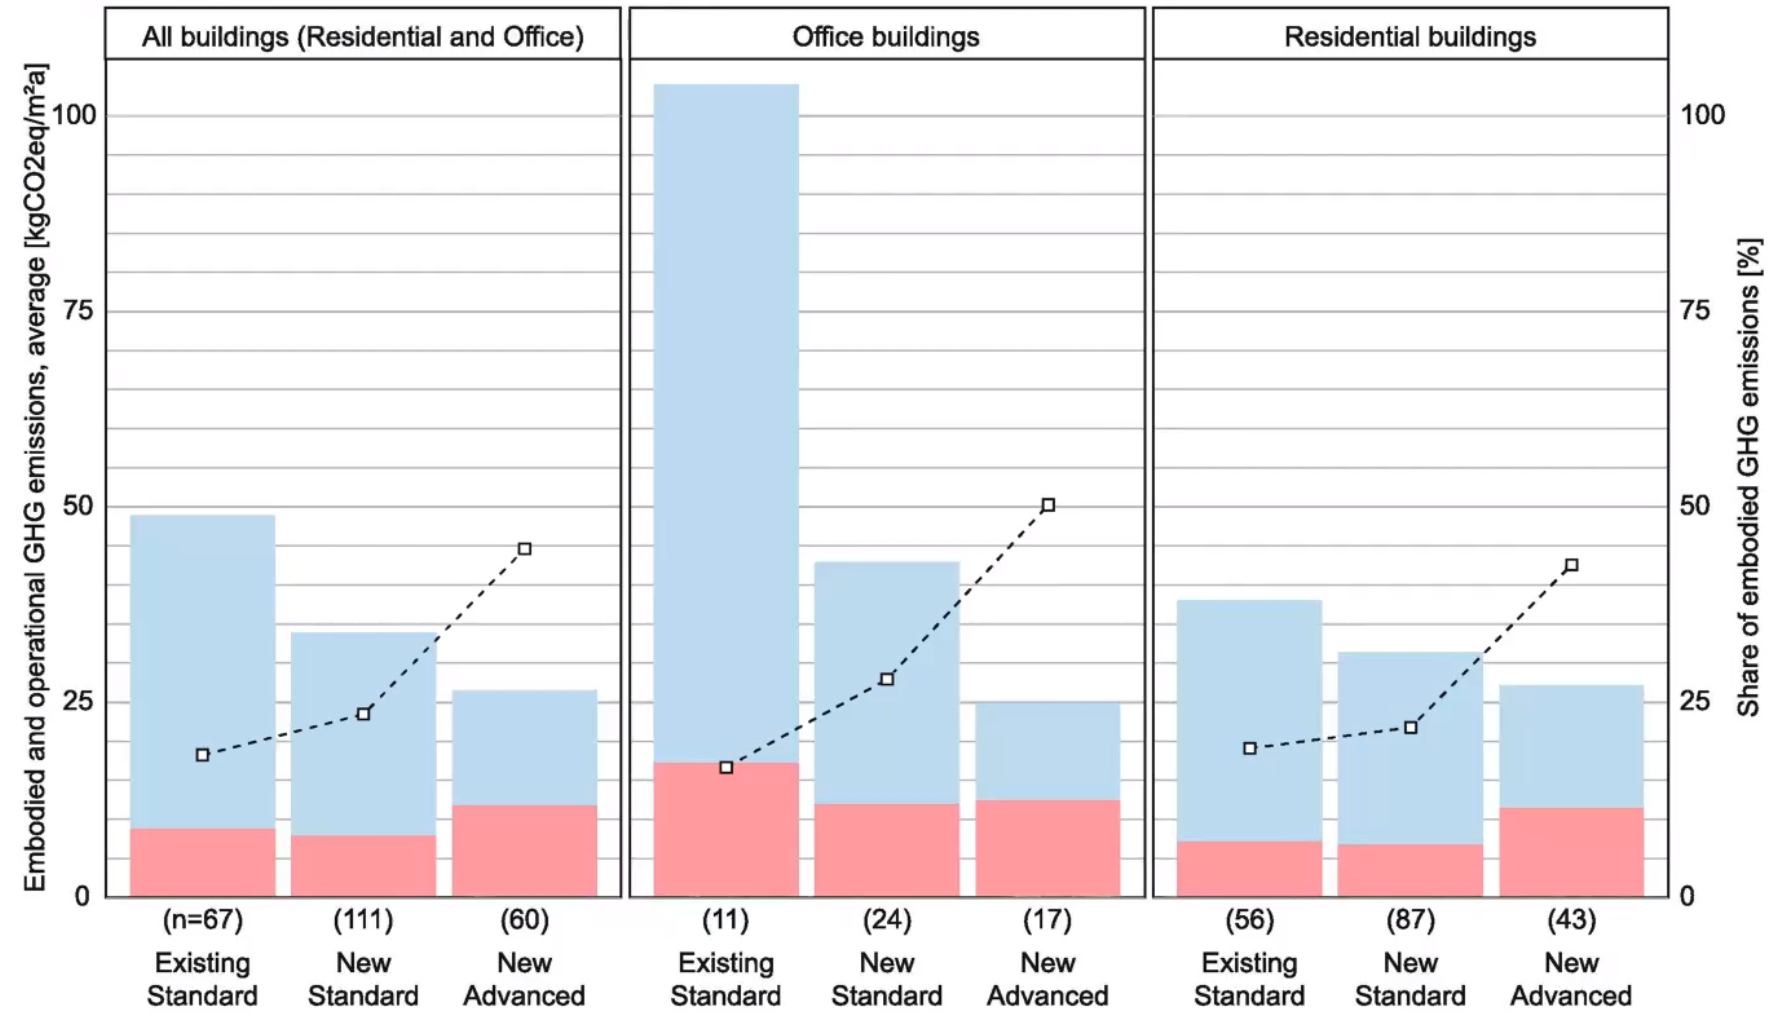
\includegraphics[width=0.7\linewidth]{../images/8-embodied-operational-trends.png}
		\caption{Global trends in embodied and operational life cycle emissions}
		\label{fig:8-embodied-operational-trends}
	\end{figure}
	
	\ \\
	Another challenge relates to other \textbf{environmental pressures caused by the building sector, beyond climate change effects}. Resource extraction for construction materials, land use for buildings, fresh water use, fine dust emissions, plastic waste, are causing important pressure on our planet in terms of for example biodiversity loss, respiratory effects, shortages in fresh water, and acidification of the ocean. 
	\\
	For many of these resources, we are currently beyond the planetary boundaries. Or, in short, \textbf{our ecological footprint is beyond the Earth’s carrying capacity}. There is hence an urgent need to further rethink the building sector to reduce our ecological footprint. 
	
	\subsubsection{Life Cycle Analysis}
	
	There is no simple and straightforward solution available to solve the various challenges the construction sector is facing to reduce its environmental impact. A combination of steps and strategies will be required to enable a further transition of our buildings and cities.
	\\
	To avoid burden shifting in time and impacts, it is important to have insights into the consequences of measures from a life cycle perspective. This means that all life cycle stages of buildings are considered when assessing their environmental impact, from the production and construction phase, over the use phase till the end-of-life phase. For buildings, the use phase will remain a very important one, seen the relatively long service life of buildings.
	
	\begin{figure}[H]
		\centering
		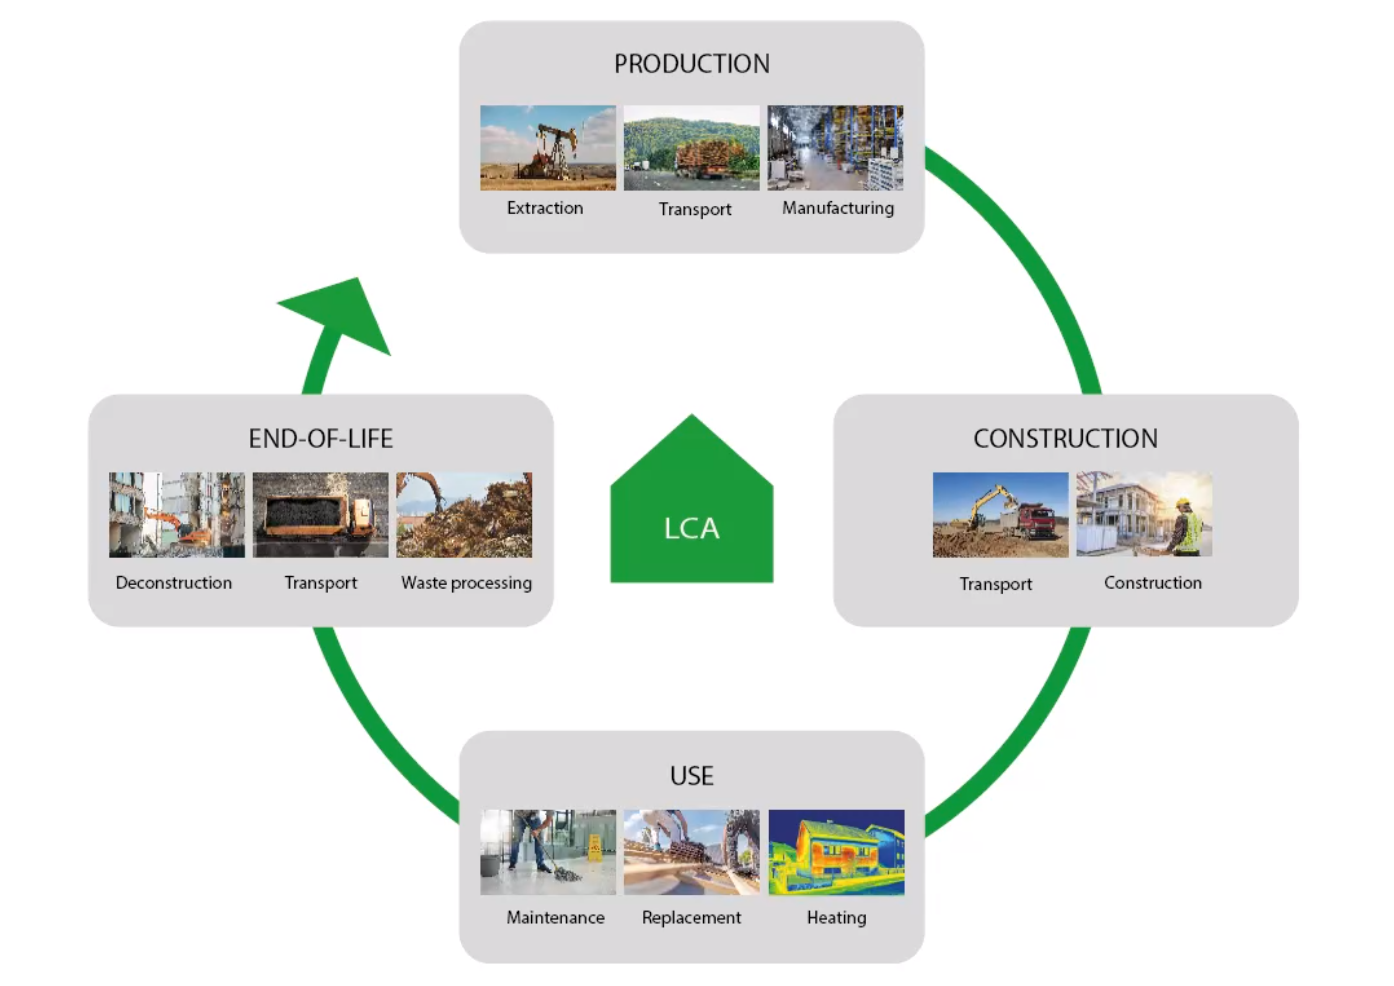
\includegraphics[width=0.7\linewidth]{../images/8-LCA}
		\caption{Life Cycle Analycis (LCA) of buildings}
		\label{fig:8-lca}
	\end{figure}
	
	\ \\
	In Life cycle assessment, typically three areas of protection are assessed: the impact on depletion of resources, the impact on quality of ecosystems and the impact on human health. The results of an LCA hence are not limited to the carbon footprint of a building, but consists of the environmental footprint. This environmental footprint covers a whole range of relevant environmental effects, such as climate change, ecotoxicity, resource depletion, carcinogenic effects, etc.
	
	\subsection{Reducing the embodied impact}
	
	Embodied impacts can be reduced by using less materials, choosing for materials with a lower environmental impact (cleaner production),
	circular building (e.g. urban mining) and extending the service life of buildings.
	\newpage
	\subsection{Sustainable construction}
	
	Thanks to the \textbf{EU policy, operational energy use of new buildings is well managed} and all stakeholders in the construction sector (architects and engineers, material producers, constructors) have enabled an important transition in the sector. The energy performance of newly built dwellings to date is much better than buildings that were built 15 years ago. The following \textbf{main challenges have been identified to further lower the environmental impact of new buildings}:
	\begin{itemize}
		\item First, \textbf{reducing the impact of the materials} by A) well-thought design of buildings to reduce the material need, B) producing and using materials with a lower environmental impact and C) circular building (high-value reuse and recycling of materials).
		\item Second, \textbf{reducing the impact of transport by sound urban planning}.
		\item Third, \textbf{reducing the land used by buildings} due to densification. This will lower the environmental footprint of buildings directly, and indirectly lower impacts due to increased public transport as public transport becomes affordable with higher densities.
	\end{itemize}
	
\end{document}